

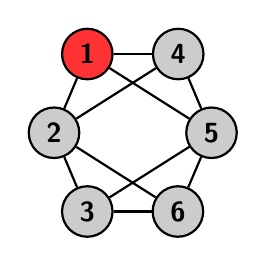
\begin{tikzpicture}[-, thick,main node/.style={circle,draw,fill=black!20,font=\sffamily\bfseries}, attack node/.style={circle,draw,fill=red!80,font=\sffamily\bfseries}] % fill=blue!20,
\node[attack node] (1) at (-0.57735,1) {1};
\node[main node] (2) at (-1,0) {2};
\node[main node] (3) at (-0.57735,-1) {3};
\node[main node] (4) at (0.57735,1) {4};
\node[main node] (5) at (1,0) {5};
\node[main node] (6) at (0.5735,-1) {6};


 \path[every node/.style={font=\sffamily\small}]
(1) edge node {} (2)
(2) edge node {} (3)
(3) edge node {} (6)
(4) edge node {} (5)
(5) edge node {} (6)
(1) edge node {} (4)


(1) edge node {} (5)
(2) edge node {} (4)
(2) edge node {} (6)
(3) edge node {} (5);



\end{tikzpicture}
